\documentclass[9pt, mathserif]{beamer}
\usepackage{ctex}
\usefonttheme{serif}
\usetheme{Berlin}
\usecolortheme{seagull}
\usepackage[utf8]{inputenc}
\usepackage{amsfonts}
\usepackage{lmodern}
\usepackage{amsmath}
\usepackage{geometry}
\usepackage{graphicx}
\usepackage{tikz}
\usepackage{url}
\usepackage{geometry}
\usepackage{bm}
\usepackage{physics}
\usepackage{float}
\usepackage{subfigure}
\usepackage{wrapfig}
\usepackage{multirow}
\usepackage{xcolor}
\usepackage{indentfirst}
\setlength{\parindent}{2em}


\title{\textbf{\textbf{}}}
\author{\textbf{宋相龙\quad Xianglong Song}}
\institute{Boling Class of Physics, School of Physics, Nankai University, Tianjin 300071, China}
\date{Jan 25, 2024}

\begin{document}
    \begin{frame}
        \titlepage
    \end{frame}
    \begin{frame}
		\frametitle{Contents} 
		\tableofcontents
	\end{frame}
    \section{Crab Nebula}
        \begin{frame}
            \frametitle{Introduction}
            The Crab Nebula (catalogue designations M1, NGC 1952, Taurus A) is a supernova remnant and pulsar wind nebula in the constellation of Taurus.

            In 2019 the Crab Nebula was observed to emit gamma rays in excess of 100 TeV, making it the first identified source beyond 100 TeV.

            \begin{figure}[t]
                \centering
                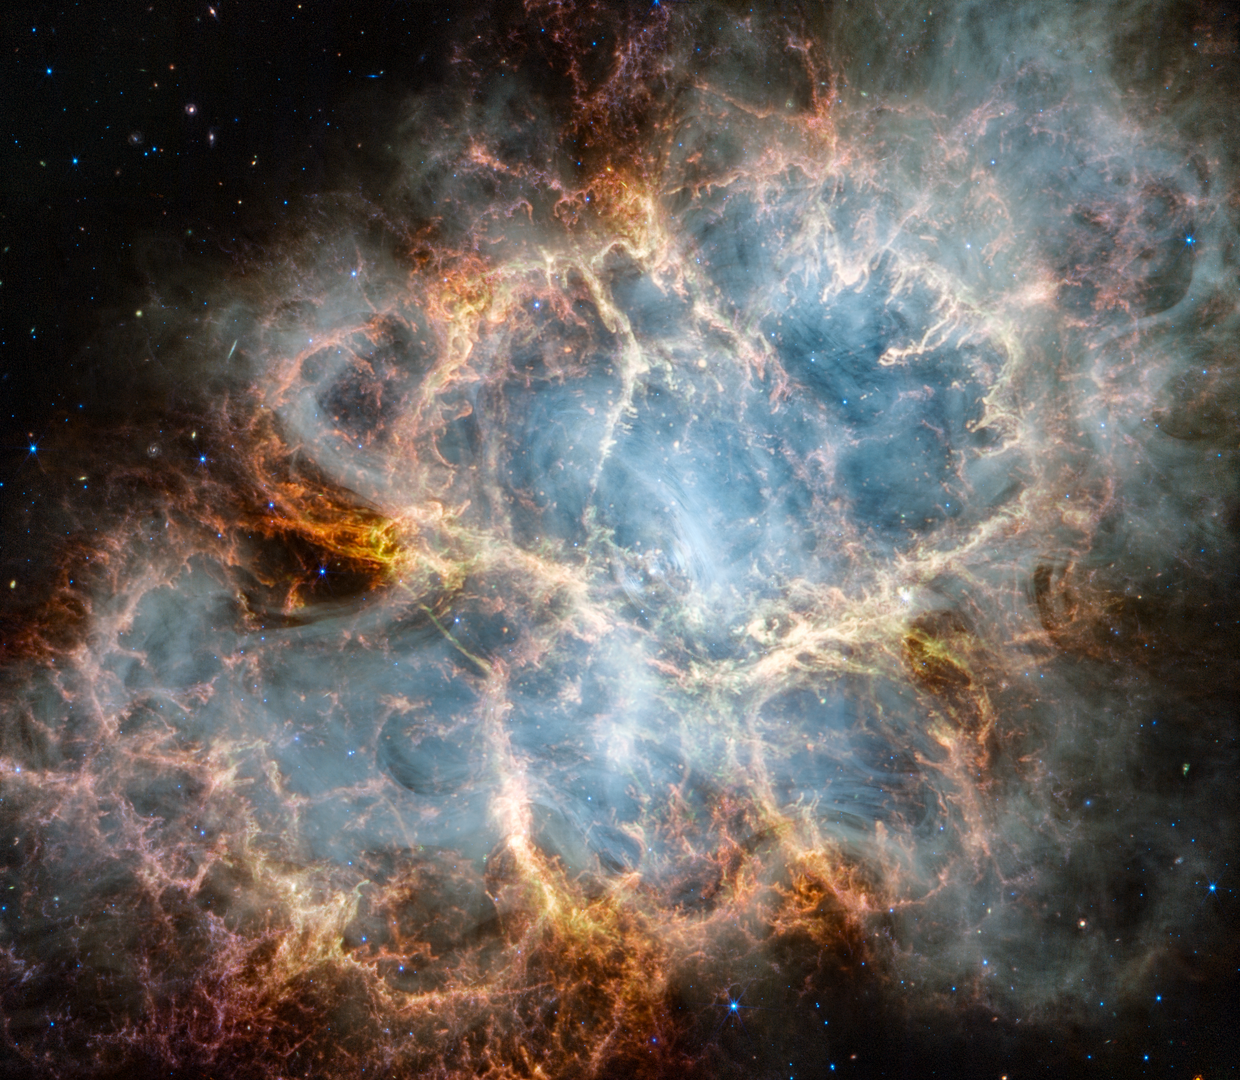
\includegraphics[\width=\textwidth]{1240px-Crab_Nebula_imaged_using_James_Webb_Space_Telescope.png}
                \caption{Crab Nebula imaged using James Webb Space Telescope in infrared via its NIRCam (Near-Infrared Camera) and MIRI (Mid-Infrared Instrument).}
            \end{figure}
        \end{frame}

    \section{References}
        \begin{frame}
            \begin{thebibliography}{1}
                \bibitem{bib1}
                {\it{高立模}}. 近代物理实验[J]. 南开大学出版社, 2006.
            \end{thebibliography}
        \end{frame}
\end{document}


